%! Author = borisdeletic
%! Date = 02/04/2023

% Preamble
\documentclass[11pt]{article}

% Packages
\usepackage{amsmath}
\usepackage{biblatex}
\usepackage{graphicx}
\usepackage{float}
\usepackage{caption}
\usepackage{subcaption}

\addbibresource{../bibliography/references.bib}
% Document
\begin{document}

    \section{Introduction}
    \subsection{Motivations (LFT)}
    Lattice field theory can be interpreted as a Bayesian sampling problem.
    Often very difficult due to multimodal likelihoods with deep topological traps.
    Topological freezing is a significant challenge which Nested Sampling helps to overcome.

    \subsection{Hamiltonian Monte Carlo (classical for LFT)}
    Describe classical HMC algorithm. \autocite{betancourt2018conceptual}

    Epsilon is the integration step size.

    Metric describes the energy level sets our HMC explores.

    \subsection{Bayesian Inference and Nested Sampling}
    Introduction to bayesian inference and Nested Sampling.\cite{Handley_polychord}

    \newpage
    \section{Constrained HMC for Nested Sampling}
    \subsection{Reflections}
    Momentum reflects off Isolikelihood contours. Visualisation similar to \cite{betancourt2016integrationtime} fig 17
    and Yallup's Nested Sampling animation.

    \subsubsection{Epsilon Halving}

    \subsection{Clustering}
    CHMC has natural clustering as the isolikelihood contour eventually separates the two modes.
    The points in each mode become isolated from eachother and each cluster evolves independently.

    \subsubsection{Local Maxima}
    Points can get stuck in local maxima and will get compressed very strongly while points in the global
    maxima will not be evolved. Therefore we need some mechanism to move points from the local max to the global max.

    To seed a new point, we can use a random live point instead of the dead point. This works, but has the problem that
    it also kills global modes which have fewer points as it implicity mixes
    points from each mode (analagous to a reaction rates problem).

    Therefore we only use a random live point for new seed on dead points that are highly compressed.

    This works to remove local maxima as the global maxima is preferred for sampling because there is more 'space'.

    \newpage
    \section{Parameter Adaption}
    There is compression of the posterior as we shrink the isolikelihood contour.
    Impossible to pick a static value for epsilon and metric which are effective for sampling
    from large posterior space and also the compressed space.
    This necessitates a dynamic adaption of our HMC parameters (epsilon, metric).
    I haven't seen this problem discussed in literature before and the following are solutions I have come up with
    using inspiration from cited papers.

    \subsection{Epsilon Dual Averaging}
    We use Nesterov Dual Averaging \cite{hoffman2011nouturn} to constantly and dynamically tune epsilon to keep a
    targeted average MH acceptance rate (0.8).
    This means our epsilon constantly is being reduced as we compress posterior.
    This is different to the original paper which terminates averaging after a burn-in period and then uses static epsilon.

    \subsection{Metric Scaling using Energy}
    As we compress posterior, the original metric explores energy level sets which become far too broad. Another way to
    say this is we are sampling momentum that are way too big for our potential function, making it look approximately uniform.
    This problem is explored in depth in this paper \cite{betancourt2016energymetric} which proposes a BFMI parameter to optimise.

    I had a different idea which uses the set of live points to estimate the variance of the constrained
    potential energy function.
    We then match the variance of the kinetic energy to the potential energy, thereby
    choosing a metric which gives an equal balance between the energies.

    I implemented both ideas in the program and my one performed better.

    \subsection{Reflection Rates for local minima}

    \newpage
    \section{Results}
    \subsection{Phi4 Theory}
    We implement Phi4 theory for Lagrangian
    \[
        S = \int{\frac{1}{2} \partial_{\mu} \phi \partial^{\mu} \phi
    -\frac{m^2}{2} \phi^2  + \frac{\lambda}{4!} \phi^4 d^4x}
    \]

    Due to path integral formalism we can interpret the (wick-rotated) action as the log-likelihood function
    for a bayesian inference problem.
    After discretising for our lattice and redefining some parameters we have the following action.
    \[
        S = \sum_{x \in \Lambda} \left[ V(\phi) - 2\kappa \sum_{\mu}{\phi(x)\phi(x+\mu)} \right]
    \]
    \[
        V(\phi) = \lambda (\phi^2 - 1)^2 + \phi^2
    \]

    This action is in the same universality class as the Ising model and exhibits a phase transition
    in $\kappa$ going from unimodal to bimodal. We plot the contours and gradient of this action
    to show the bimodal loglikelihood function.

    \begin{figure}[H]
        \centering
        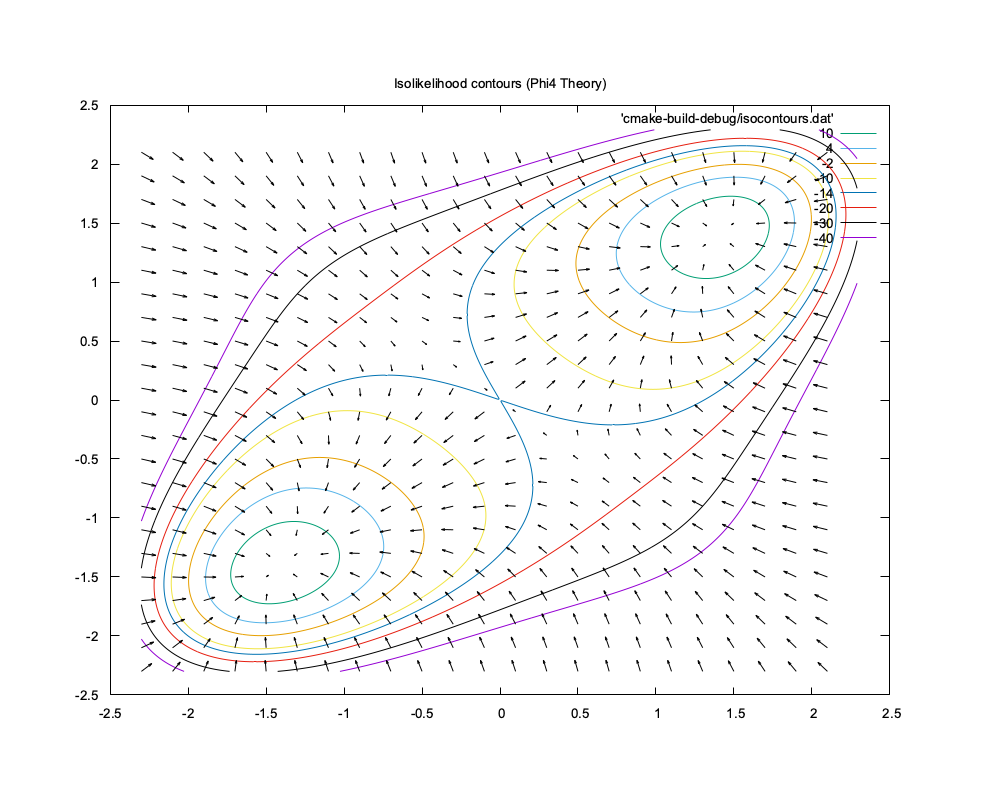
\includegraphics[width=0.75\linewidth]{../figures/phi4_isocontours}
        \caption{Phi4 Theory Isolikelihood Contours and Gradient}
        \label{fig:phi4contour}
    \end{figure}

    \begin{figure}[H]
        \centering
        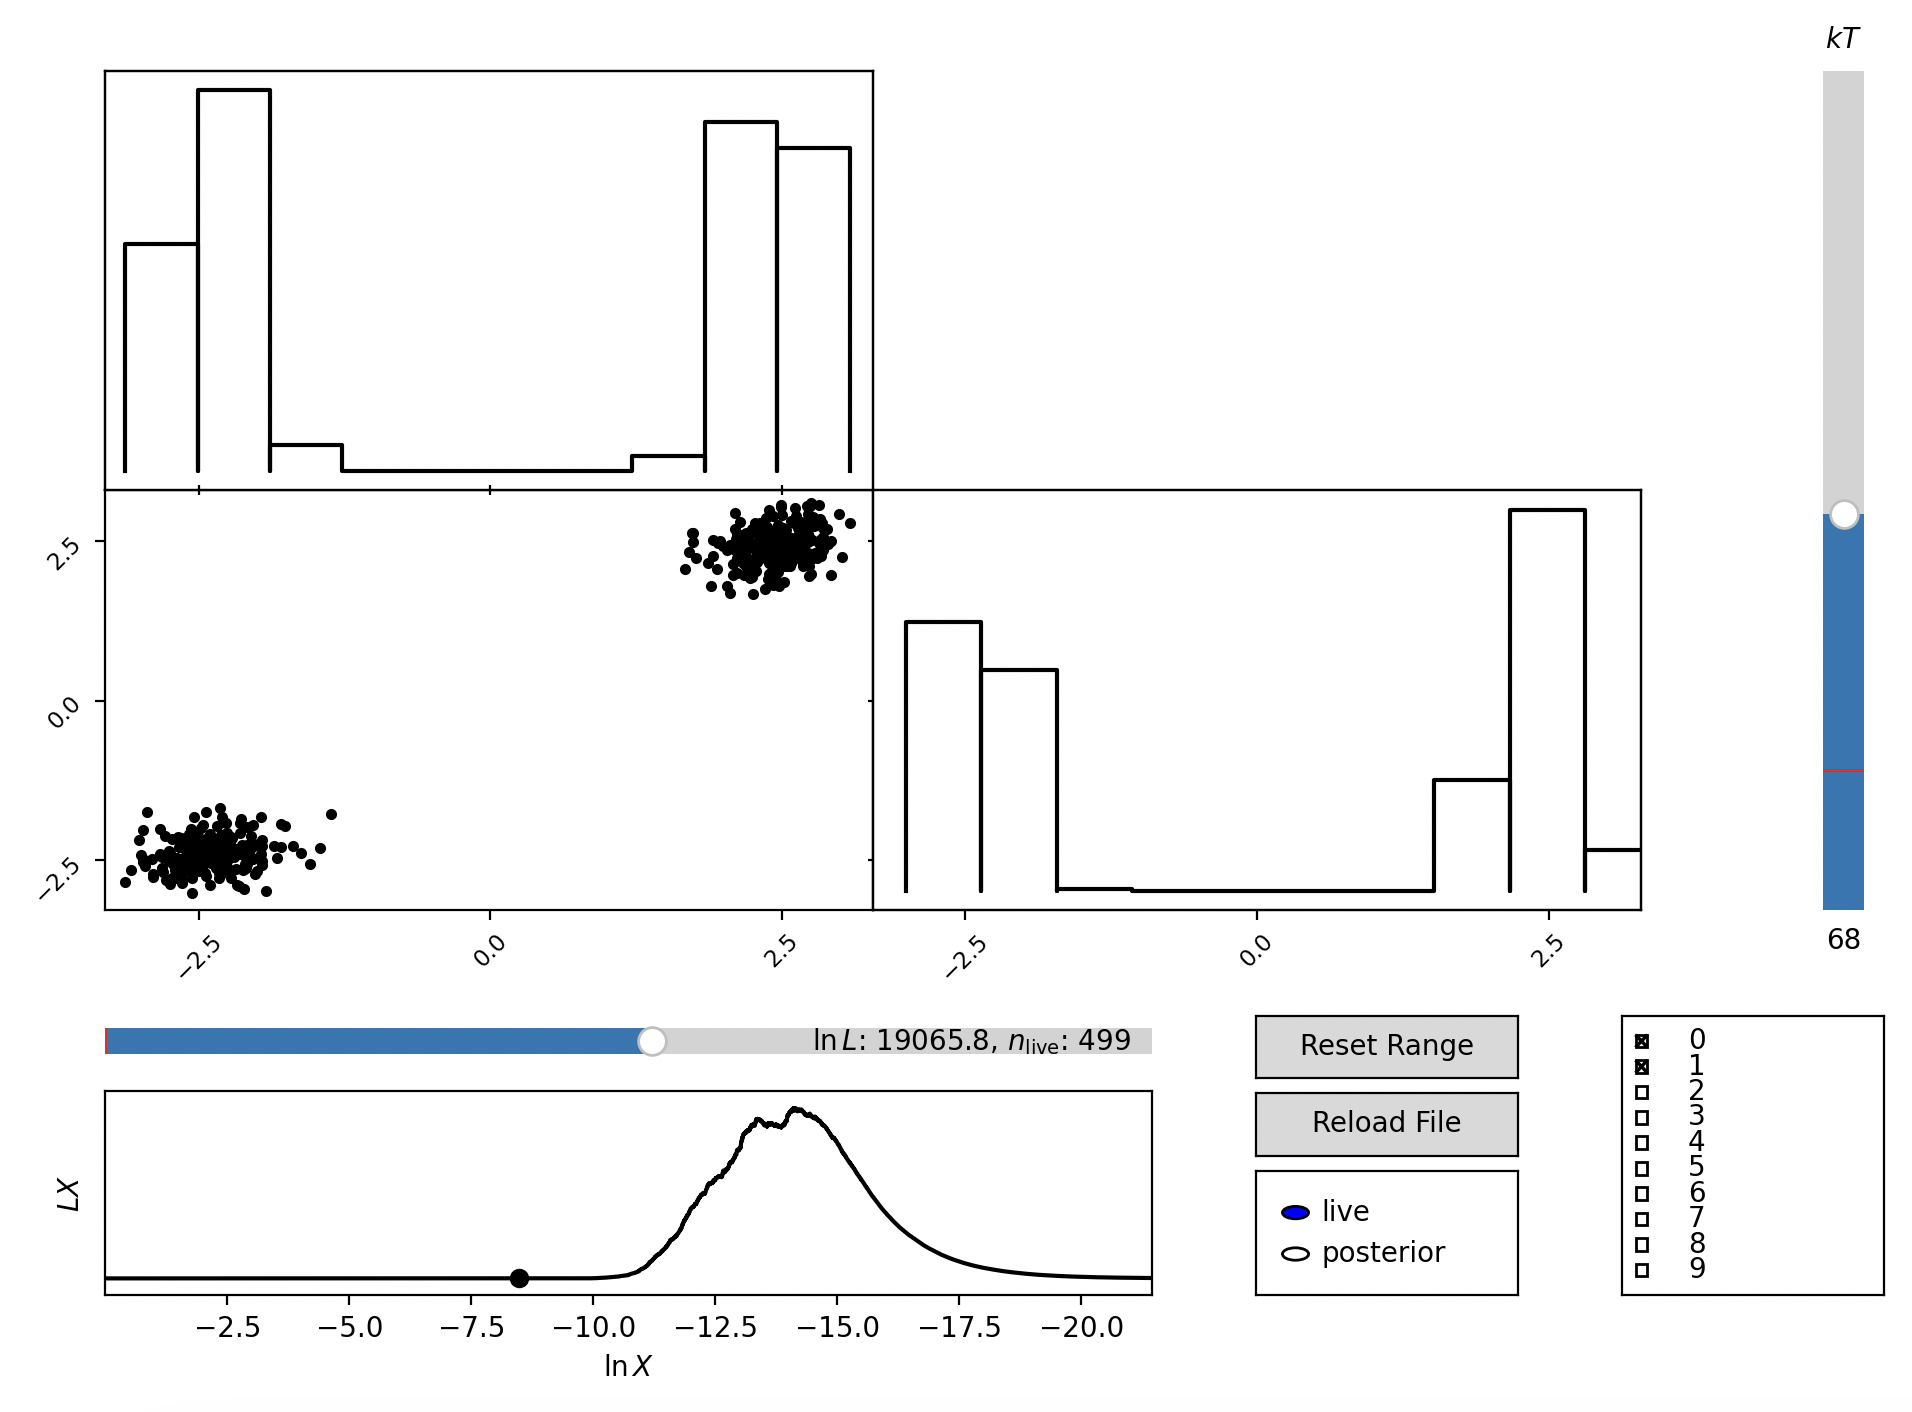
\includegraphics[width=0.75\linewidth]{../figures/phi4_anesthetic}
        \caption{Nested Sampling for Phi4 Theory correctly finds both modes}
        \label{fig:phi4anesthetic}
    \end{figure}

    \subsubsection{Correlation Functions}
    Correlation functions are the key observable which allow us to perform QFT measurements in a statistical framework.
    We define the equal-time (position) correlation function for $\phi^4$ theory as
    \[
        C(x_1, x_2) = \langle \phi(x_1) \phi(x_2) \rangle
    \]
    Where $\langle . \rangle$ represents the ensemble average.
    Exploiting the rotational and translation symmetry of $\phi^4$ theory, we can fully characterise this function
    in terms of the distance $r$ between two points along the horizontal or vertical axis of the lattice.
    \[
        C(r) = \langle \phi(x') \phi(x' + r) \rangle
    \]
    Where we also average over all lattice points $x'$.
    Calculating this function directly is prohibitively expensive and grows as $O(L^3)$, where $L$ is the lattice dimension\\

    To speed up this computation we use a discrete fourier transform and an application of the convolution theorem. \cite{Ruge_1994}
    In the continuous limit, the correlation function over all lattice points for a single ensemble state $n$ can be written as
    \[
        C_n(r) = \int_{-\infty}^{\infty} \phi(x) \phi(x - r) dx
    \]
    We apply the convolution theorem and inverse fourier transform to write
    \[
        C_n(r) = \mathcal{F}^{-1} \left( | \widetilde{\phi(k)} |^2 \right)
    \]
    Which we can compute with complexity $O(L^2 \log(L))$.



    \subsection{Topological Trap}
    We investigate the results on a likelihood function with a topological trap
    consisting of a wide local maximum basin, and a narrow global maximum.

    \[
        \log \mathcal{L} = -x^2 + a e^{-(x-\mu)^2}
    \]

    \begin{figure}[H]
        \centering
        \begin{subfigure}[b]{0.35\linewidth}
            \centering
            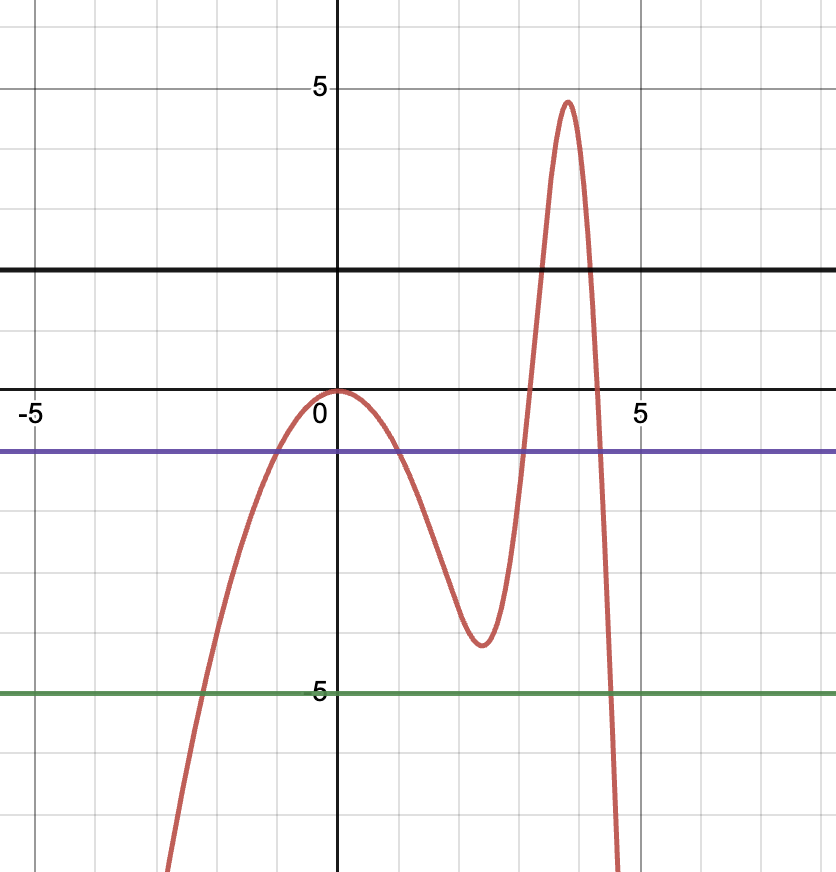
\includegraphics[width=\linewidth]{../figures/topotrap/function}
            \caption{Topological Trap Function with Isolikelihood slices}
        \end{subfigure}
        \begin{subfigure}[b]{0.55\linewidth}
            \centering
            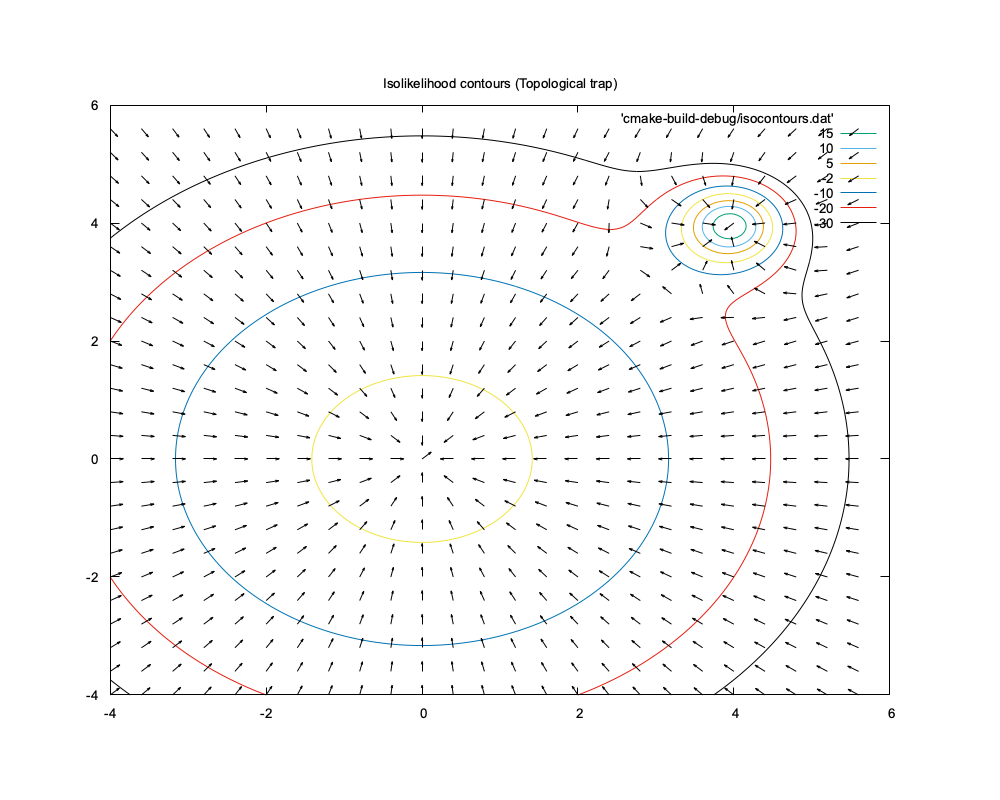
\includegraphics[width=\linewidth]{../figures/topotrap/contour}
            \caption{2D view of function with contours and gradient}
        \end{subfigure}
        \label{dig:topotrap_function}
    \end{figure}

    We can see the CHMC nested sampling successfully solves this case.
    \begin{figure}[H]
        \centering
        \begin{subfigure}[b]{0.3\linewidth}
            \centering
            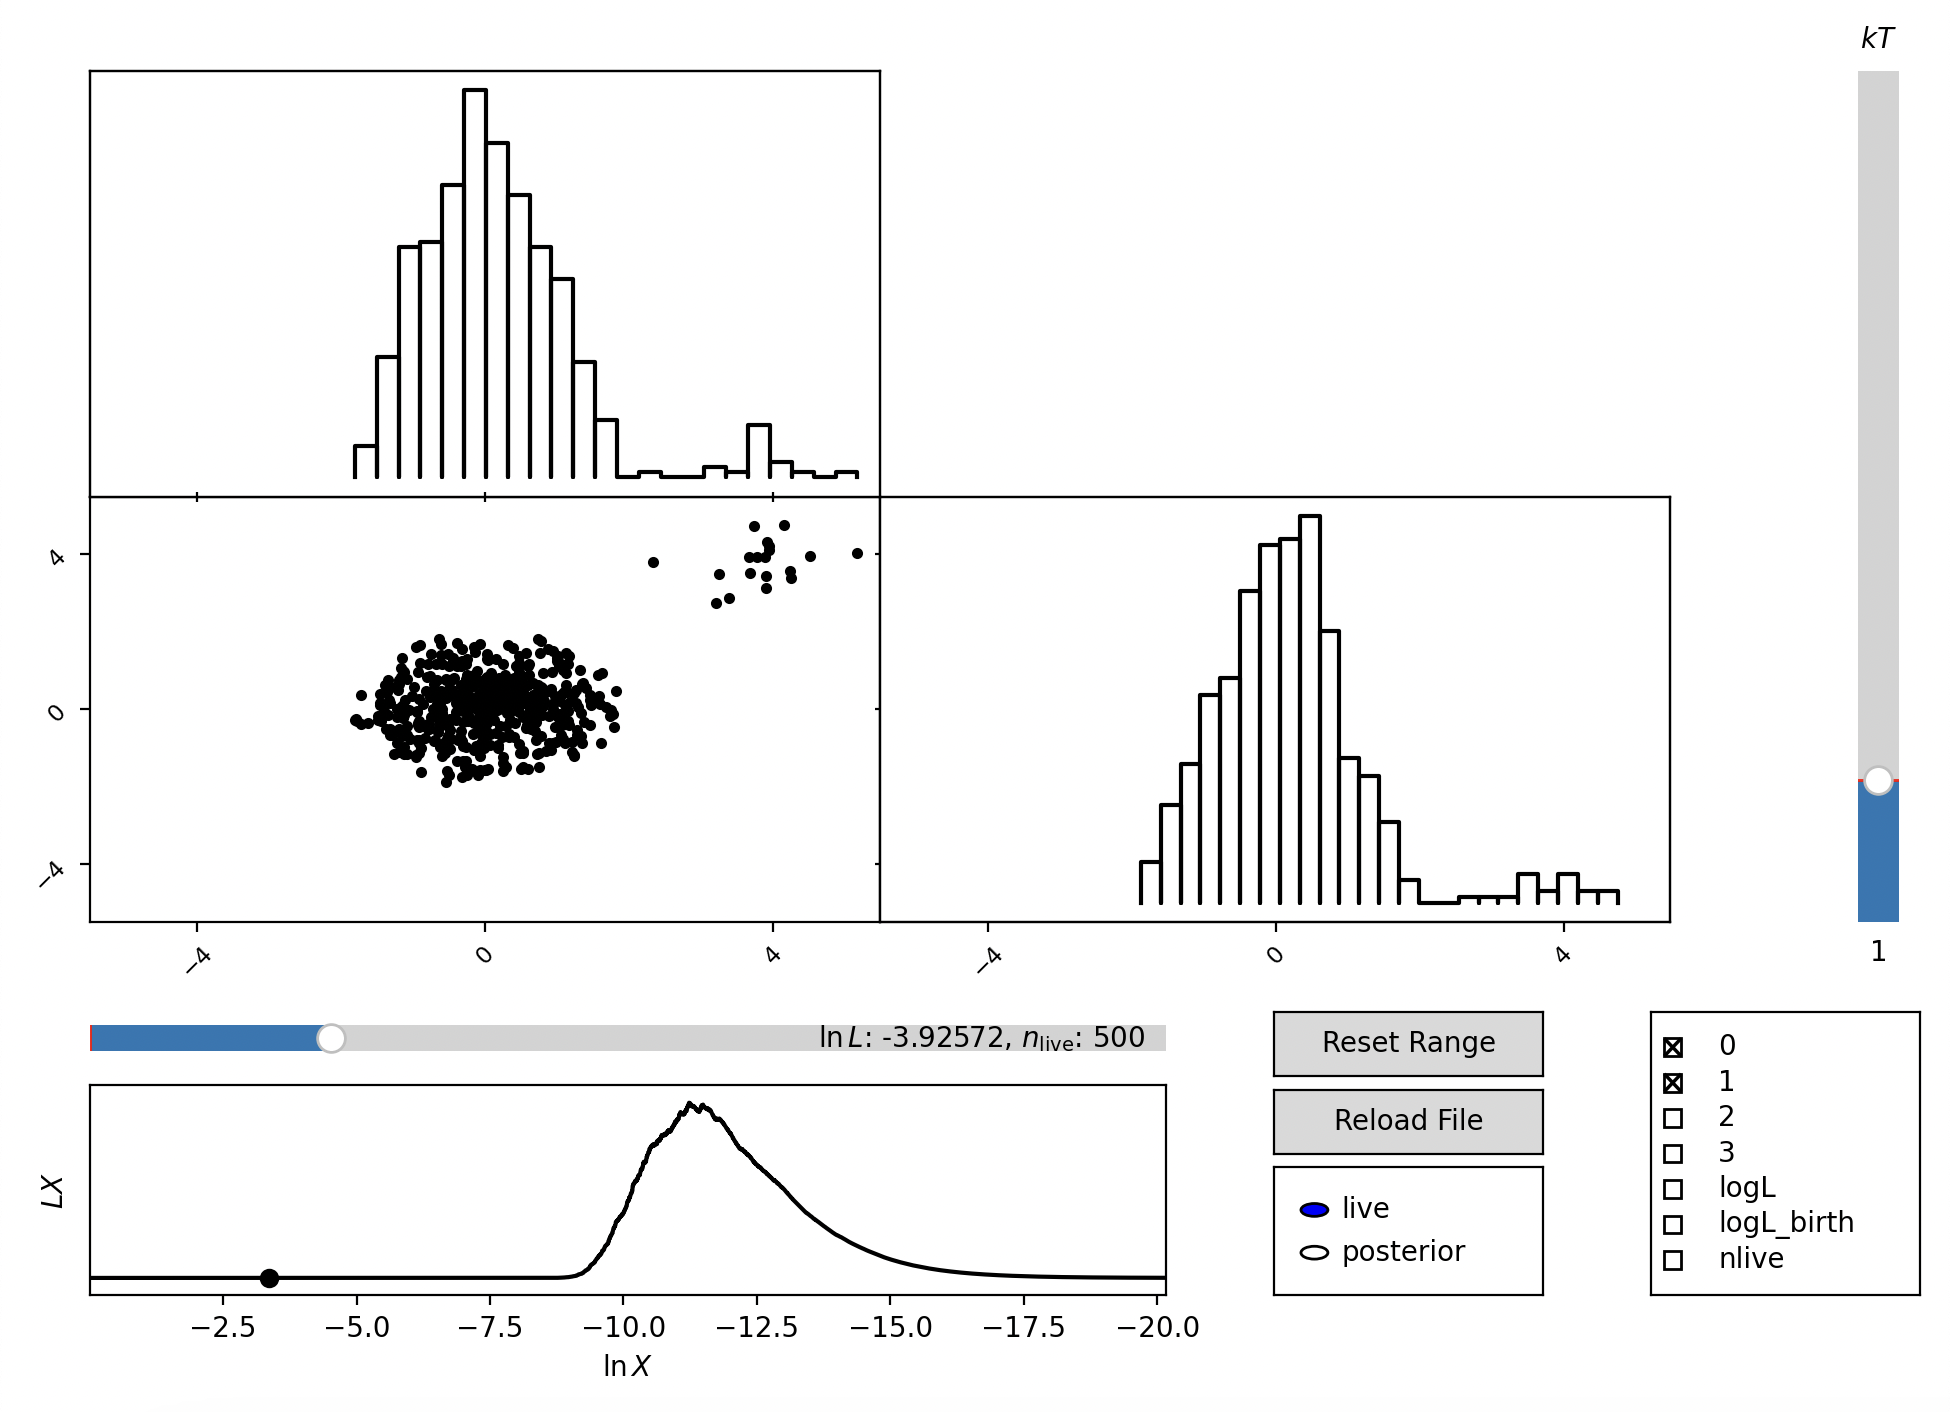
\includegraphics[width=\linewidth]{../figures/topotrap/NS1}
            \caption{Majority in local max}
        \end{subfigure}
        \begin{subfigure}[b]{0.3\linewidth}
            \centering
            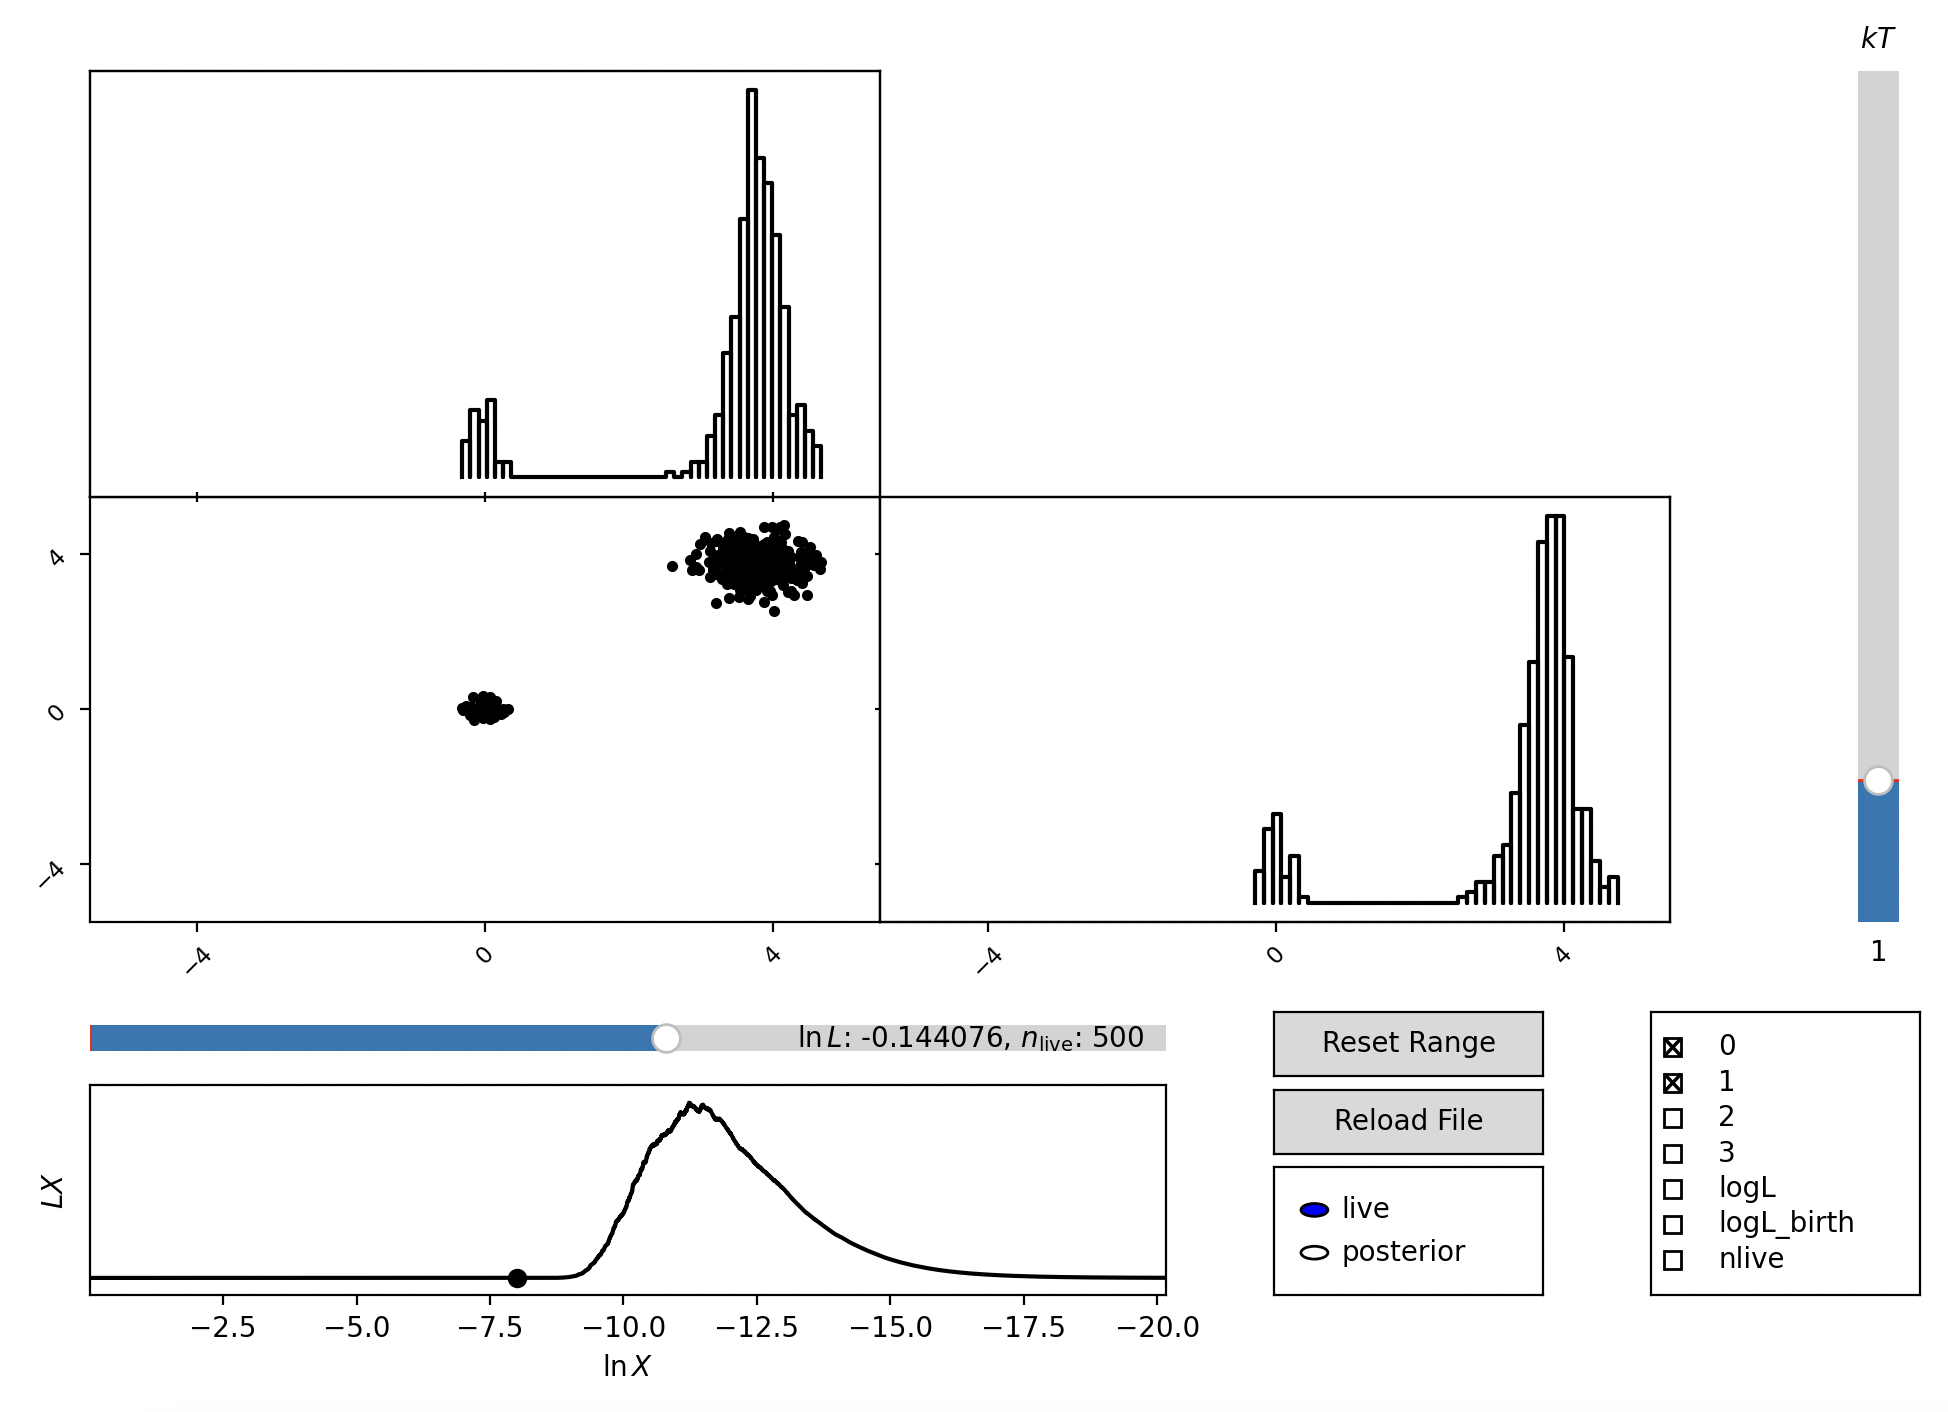
\includegraphics[width=\linewidth]{../figures/topotrap/NS2}
            \caption{Points move to global max}
        \end{subfigure}
        \begin{subfigure}[b]{0.3\linewidth}
            \centering
            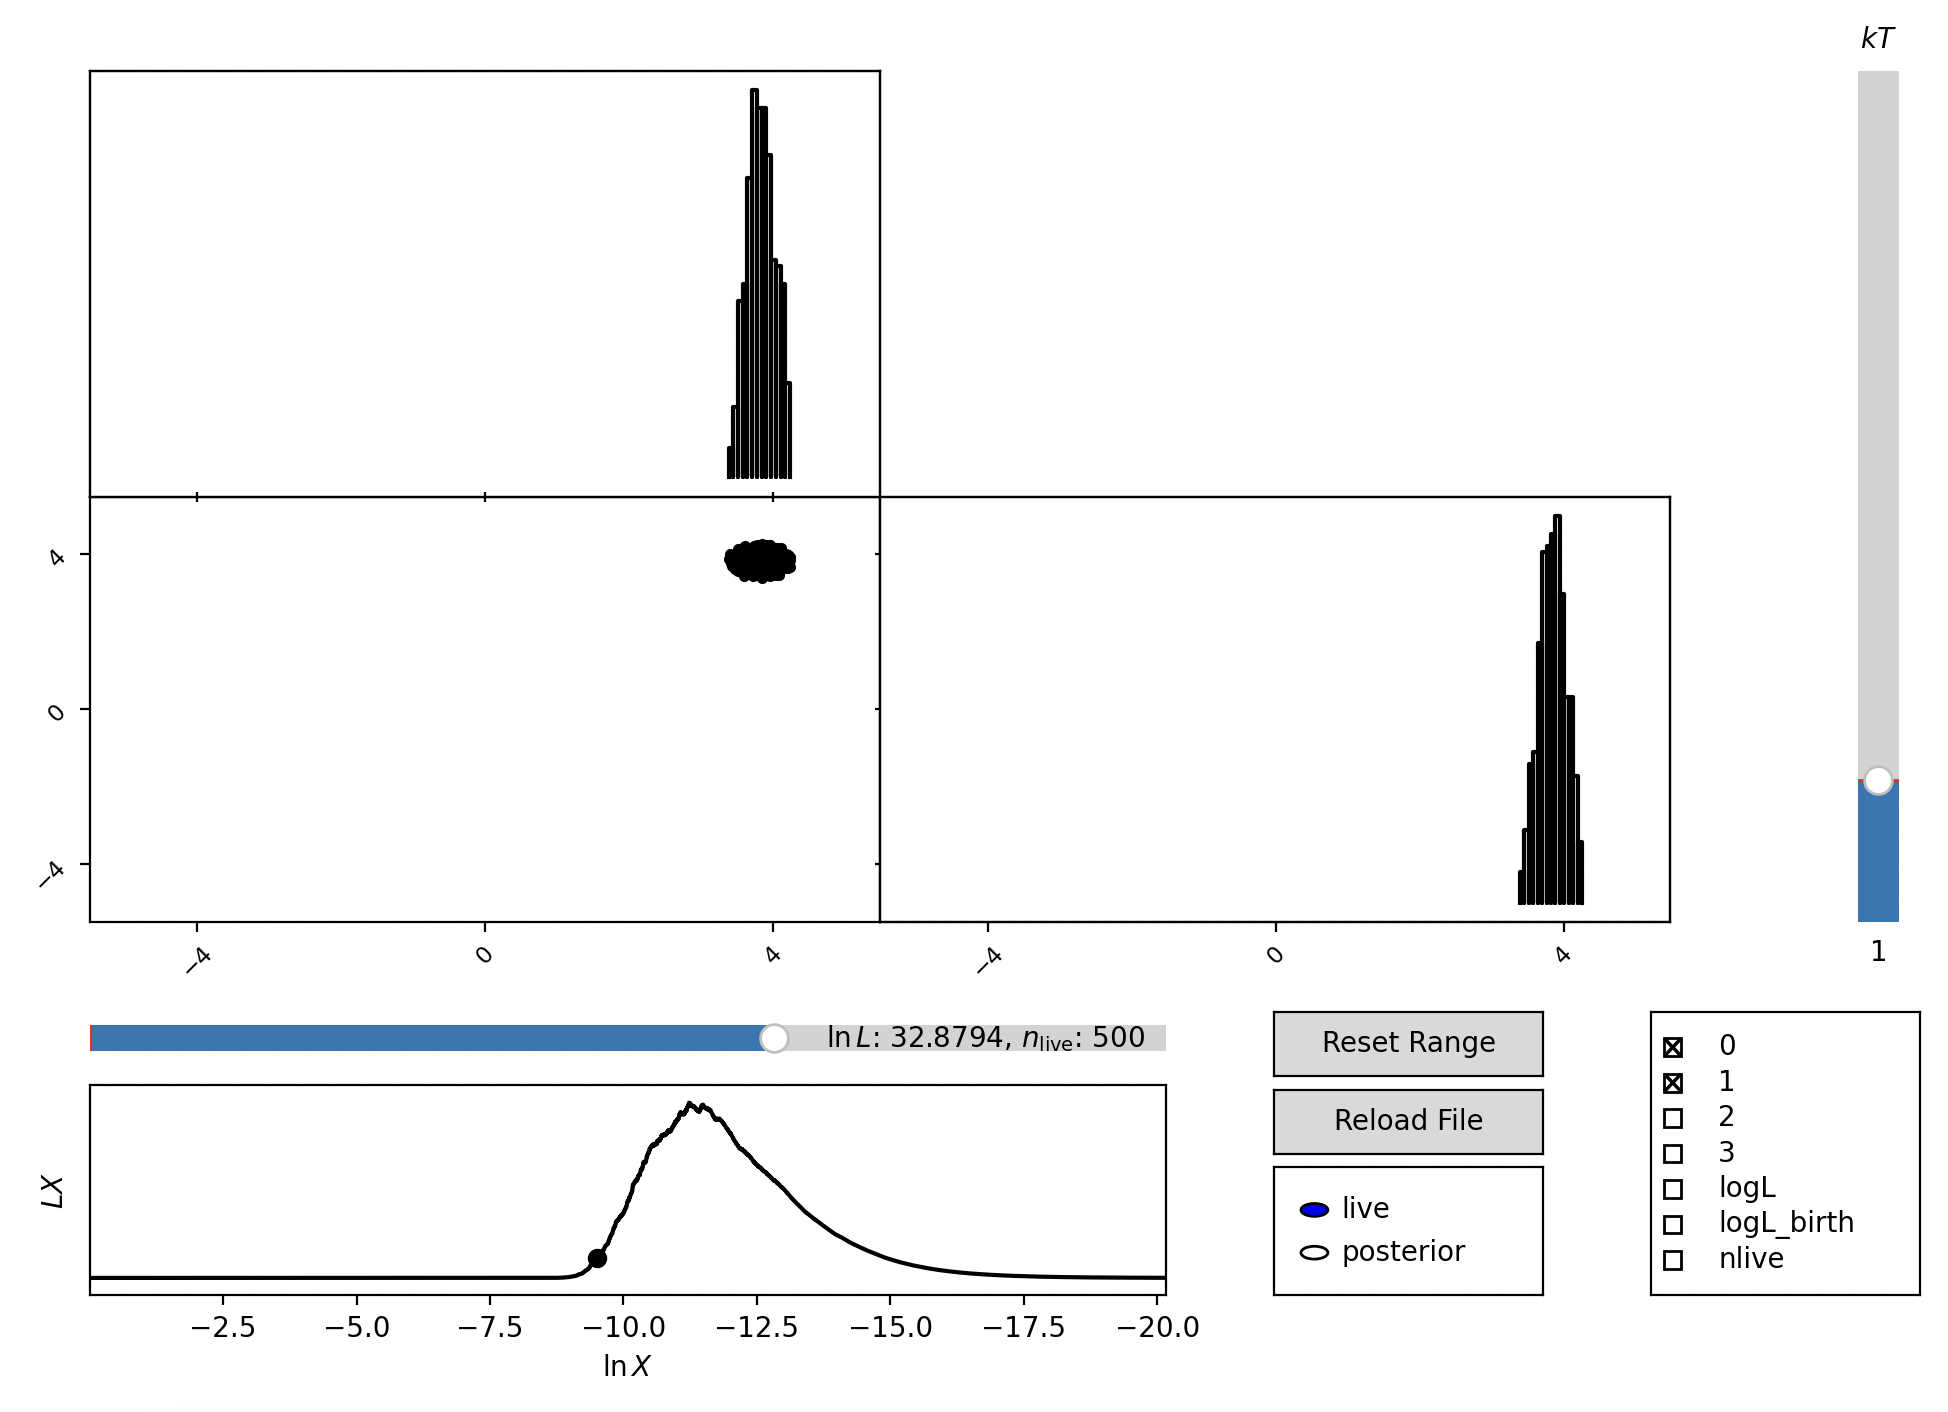
\includegraphics[width=\linewidth]{../figures/topotrap/NS3}
            \caption{Sampled past local max}
        \end{subfigure}
        \label{dig:topotrap_ns}
    \end{figure}


    \subsection{Performance}
    No parallelization implemented yet.
    Phi4 Theory benchmark runs on 20x20 lattice (400 dimension) in ~4min on single core of MacbookPro,
    taking about 7000 Nested Sampling steps to converge (0.01 precision criterion).

    Number of likelihood calls per nested sampling step is independent of dimension.

    The same Phi4 likelihood function run on Polychord does not converge within one hour on all cores.

    \newpage
    \appendix
    \section{Code Design}
    \subsection{Interfaces}
    Present UML diagram for code base class structure
    \subsection{Unit Tests}
    Implemented unit test framework with (currently 12) unit tests to raise confidence of correctness.
    \section{Auto Differentiation}
    All likelihood functions used have analytic gradients currently. Code has Enzyme support which contains
    functionality for auto-differentiation (untested). \\

    $S = &\,\sum\limits_{x \in \Lambda} \Biggl[-2\kappa \sum\limits_{\mu=1}^d
    \phi(x) \phi(x+\hat{\mu}) + (1 - 2\lambda) \phi(x)^2 + \lambda \phi(x)^4 \Biggr]$


    \printbibliography
\end{document}